\documentclass[14pt]{extbook}
\usepackage{multicol, enumerate, enumitem, hyperref, color, soul, setspace, parskip, fancyhdr} %General Packages
\usepackage{amssymb, amsthm, amsmath, latexsym, units, mathtools} %Math Packages
\everymath{\displaystyle} %All math in Display Style
% Packages with additional options
\usepackage[headsep=0.5cm,headheight=12pt, left=1 in,right= 1 in,top= 1 in,bottom= 1 in]{geometry}
\usepackage[usenames,dvipsnames]{xcolor}
\usepackage{dashrule}  % Package to use the command below to create lines between items
\newcommand{\litem}[1]{\item#1\hspace*{-1cm}\rule{\textwidth}{0.4pt}}
\pagestyle{fancy}
\lhead{Makeup Progress Quiz 3}
\chead{}
\rhead{Version ALL}
\lfoot{1648-1753}
\cfoot{}
\rfoot{Summer C 2021}
\begin{document}

\begin{enumerate}
\litem{
Choose the equation of the function graphed below.
\begin{center}
    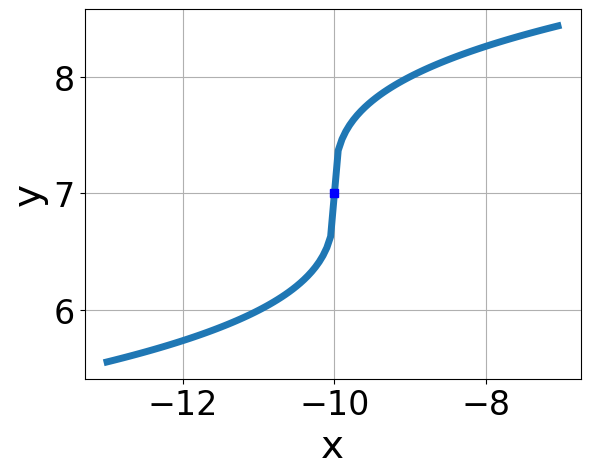
\includegraphics[width=0.5\textwidth]{../Figures/radicalGraphToEquationA.png}
\end{center}
\begin{enumerate}[label=\Alph*.]
\item \( f(x) = \sqrt{x - 10} + 7 \)
\item \( f(x) = - \sqrt{x - 10} + 7 \)
\item \( f(x) = - \sqrt{x + 10} + 7 \)
\item \( f(x) = \sqrt{x + 10} + 7 \)
\item \( \text{None of the above} \)

\end{enumerate} }
\litem{
Choose the graph of the equation below.\[ f(x) = - \sqrt{x - 12} - 6 \]\begin{enumerate}[label=\Alph*.]
\begin{multicols}{2}\item 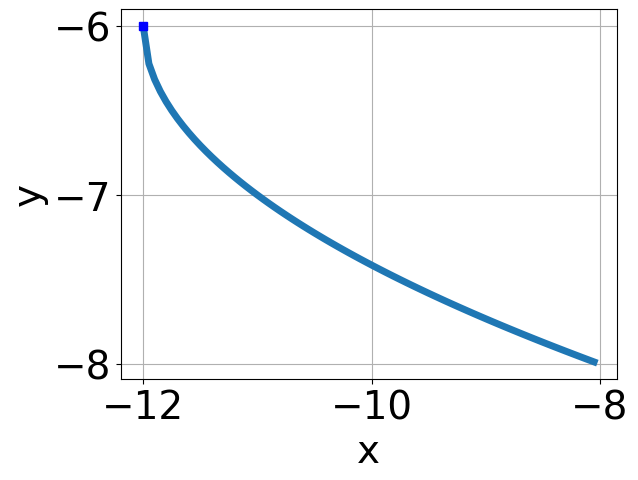
\includegraphics[width = 0.3\textwidth]{../Figures/radicalEquationToGraphCopyAA.png}\item 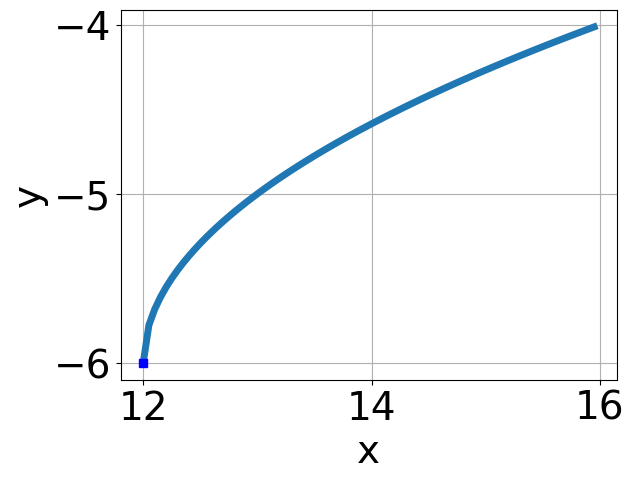
\includegraphics[width = 0.3\textwidth]{../Figures/radicalEquationToGraphCopyBA.png}\item 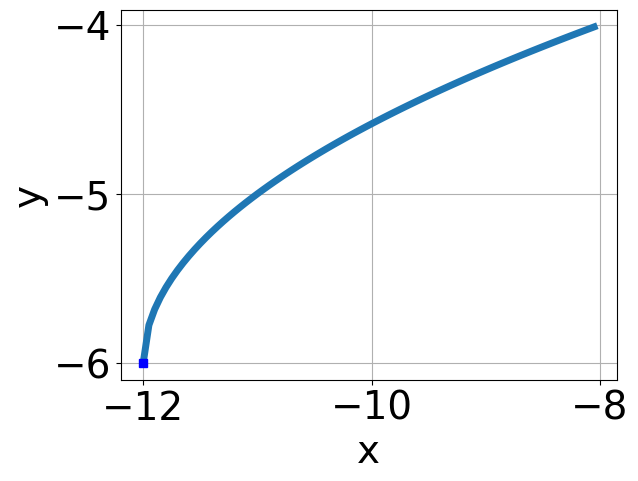
\includegraphics[width = 0.3\textwidth]{../Figures/radicalEquationToGraphCopyCA.png}\item 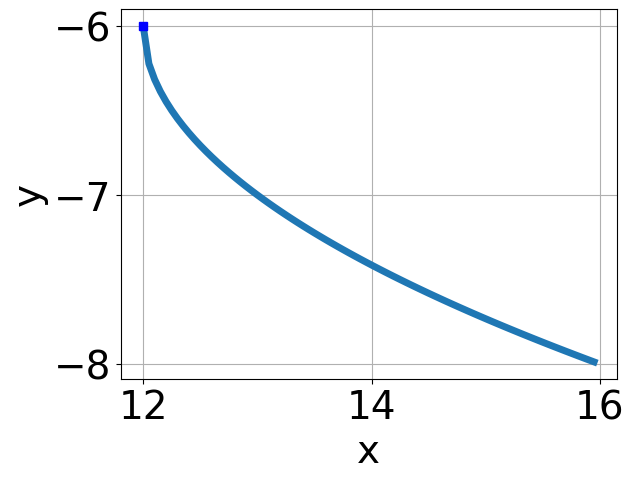
\includegraphics[width = 0.3\textwidth]{../Figures/radicalEquationToGraphCopyDA.png}\end{multicols}\item None of the above.
\end{enumerate} }
\litem{
What is the domain of the function below?\[ f(x) = \sqrt[8]{-4 x - 5} \]\begin{enumerate}[label=\Alph*.]
\item \( (-\infty, a], \text{ where } a \in [-3.4, -1.1] \)
\item \( (-\infty, a], \text{where } a \in [-1.1, 1.3] \)
\item \( (-\infty, \infty) \)
\item \( [a, \infty), \text{where } a \in [-3.4, -1] \)
\item \( [a, \infty), \text{where } a \in [-1.2, -0.3] \)

\end{enumerate} }
\litem{
Solve the radical equation below. Then, choose the interval(s) that the solution(s) belongs to.\[ \sqrt{54 x^2 + 56} - \sqrt{-111 x} = 0 \]\begin{enumerate}[label=\Alph*.]
\item \( x_1 \in [0.68, 1.17] \text{ and } x_2 \in [0.6,2.5] \)
\item \( x \in [-1.4,-1.13] \)
\item \( x_1 \in [-1.4, -1.13] \text{ and } x_2 \in [-1.2,-0.7] \)
\item \( \text{All solutions lead to invalid or complex values in the equation.} \)
\item \( x \in [-0.96,-0.86] \)

\end{enumerate} }
\litem{
Choose the equation of the function graphed below.
\begin{center}
    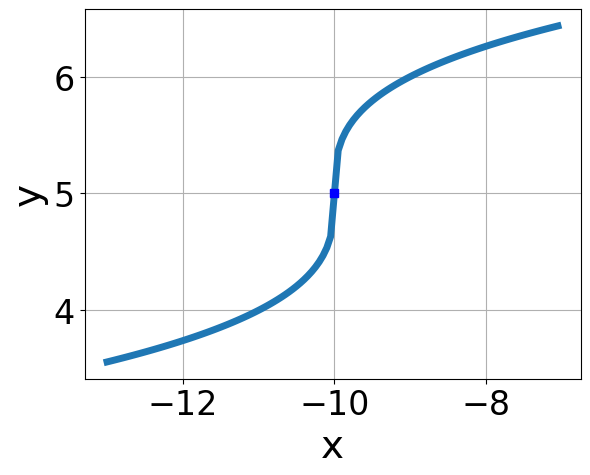
\includegraphics[width=0.5\textwidth]{../Figures/radicalGraphToEquationCopyA.png}
\end{center}
\begin{enumerate}[label=\Alph*.]
\item \( f(x) = \sqrt[3]{x - 10} + 5 \)
\item \( f(x) = - \sqrt[3]{x + 10} + 5 \)
\item \( f(x) = \sqrt[3]{x + 10} + 5 \)
\item \( f(x) = - \sqrt[3]{x - 10} + 5 \)
\item \( \text{None of the above} \)

\end{enumerate} }
\litem{
Solve the radical equation below. Then, choose the interval(s) that the solution(s) belongs to.\[ \sqrt{-5 x + 3} - \sqrt{-2 x - 8} = 0 \]\begin{enumerate}[label=\Alph*.]
\item \( x_1 \in [-1.3, 1.9] \text{ and } x_2 \in [2.67,6.67] \)
\item \( \text{All solutions lead to invalid or complex values in the equation.} \)
\item \( x \in [-3.5,-0.8] \)
\item \( x \in [3,4.1] \)
\item \( x_1 \in [-5.8, -3.9] \text{ and } x_2 \in [-1.4,3.6] \)

\end{enumerate} }
\litem{
Solve the radical equation below. Then, choose the interval(s) that the solution(s) belongs to.\[ \sqrt{6 x^2 - 16} - \sqrt{4 x} = 0 \]\begin{enumerate}[label=\Alph*.]
\item \( x_1 \in [-1.44, -1.16] \text{ and } x_2 \in [-5,3] \)
\item \( x \in [-1.44,-1.16] \)
\item \( x_1 \in [0.82, 1.38] \text{ and } x_2 \in [-5,3] \)
\item \( \text{All solutions lead to invalid or complex values in the equation.} \)
\item \( x \in [1.48,2.32] \)

\end{enumerate} }
\litem{
Solve the radical equation below. Then, choose the interval(s) that the solution(s) belongs to.\[ \sqrt{7 x - 5} - \sqrt{8 x + 5} = 0 \]\begin{enumerate}[label=\Alph*.]
\item \( x_1 \in [-1.1, -0.15] \text{ and } x_2 \in [-1.29,1.71] \)
\item \( x_1 \in [-10.3, -9.84] \text{ and } x_2 \in [-1.29,1.71] \)
\item \( x \in [-10.3,-9.84] \)
\item \( \text{All solutions lead to invalid or complex values in the equation.} \)
\item \( x \in [-0.29,0.45] \)

\end{enumerate} }
\litem{
Choose the graph of the equation below.\[ f(x) = \sqrt{x + 8} + 6 \]\begin{enumerate}[label=\Alph*.]
\begin{multicols}{2}\item 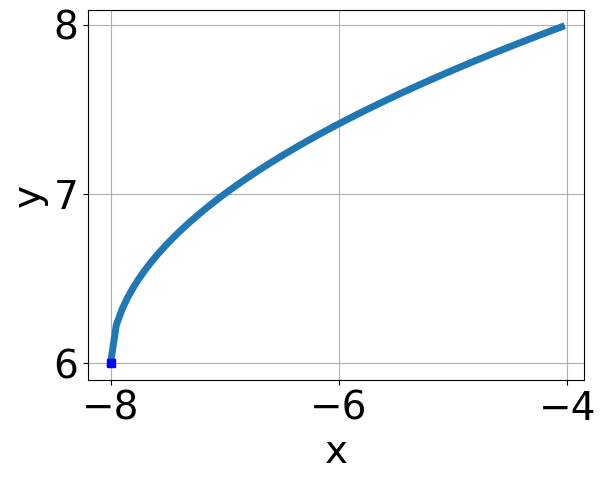
\includegraphics[width = 0.3\textwidth]{../Figures/radicalEquationToGraphAA.png}\item 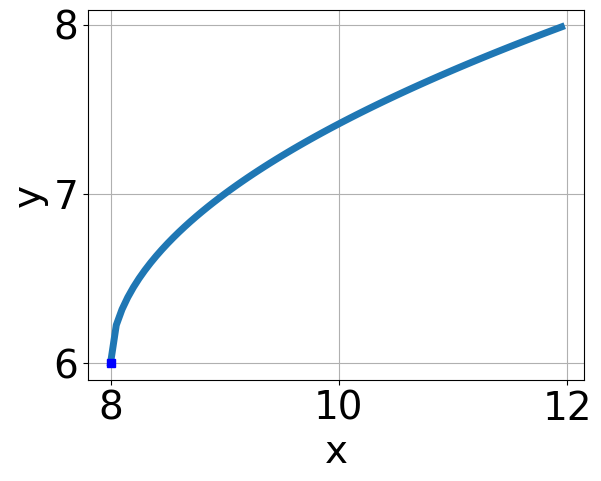
\includegraphics[width = 0.3\textwidth]{../Figures/radicalEquationToGraphBA.png}\item 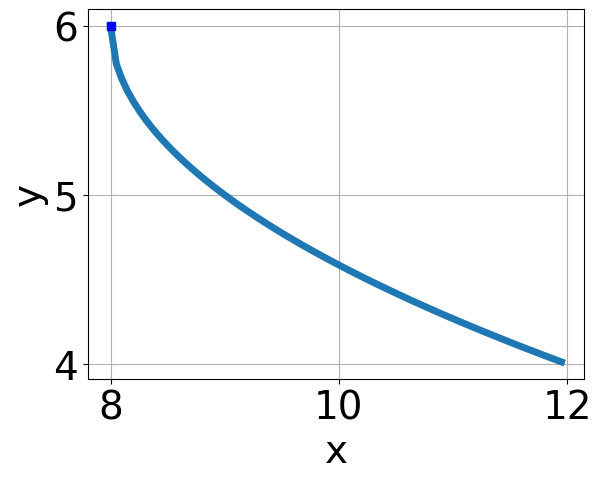
\includegraphics[width = 0.3\textwidth]{../Figures/radicalEquationToGraphCA.png}\item 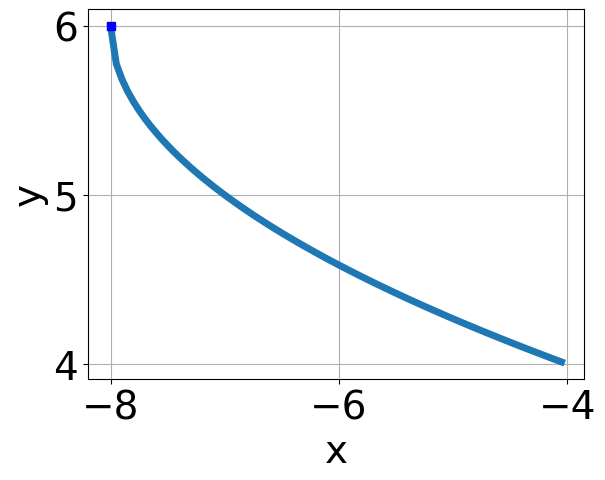
\includegraphics[width = 0.3\textwidth]{../Figures/radicalEquationToGraphDA.png}\end{multicols}\item None of the above.
\end{enumerate} }
\litem{
What is the domain of the function below?\[ f(x) = \sqrt[4]{7 x - 8} \]\begin{enumerate}[label=\Alph*.]
\item \( (-\infty, \infty) \)
\item \( (-\infty, a], \text{where } a \in [1.1, 1.45] \)
\item \( [a, \infty), \text{ where } a \in [1.07, 1.19] \)
\item \( [a, \infty), \text{where } a \in [0.7, 1.05] \)
\item \( (-\infty, a], \text{where } a \in [0.37, 1.01] \)

\end{enumerate} }
\litem{
Choose the equation of the function graphed below.
\begin{center}
    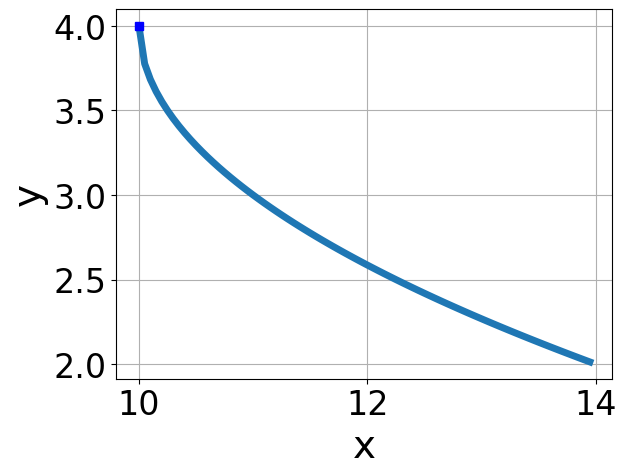
\includegraphics[width=0.5\textwidth]{../Figures/radicalGraphToEquationB.png}
\end{center}
\begin{enumerate}[label=\Alph*.]
\item \( f(x) = - \sqrt[3]{x - 10} + 4 \)
\item \( f(x) = \sqrt[3]{x - 10} + 4 \)
\item \( f(x) = \sqrt[3]{x + 10} + 4 \)
\item \( f(x) = - \sqrt[3]{x + 10} + 4 \)
\item \( \text{None of the above} \)

\end{enumerate} }
\litem{
Choose the graph of the equation below.\[ f(x) = \sqrt[3]{x - 10} + 6 \]\begin{enumerate}[label=\Alph*.]
\begin{multicols}{2}\item 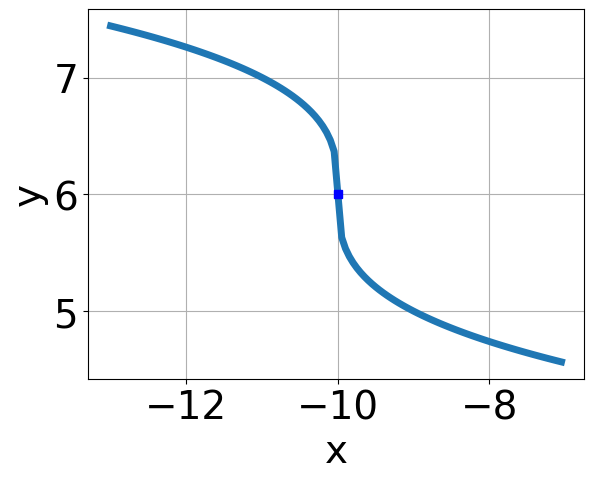
\includegraphics[width = 0.3\textwidth]{../Figures/radicalEquationToGraphCopyAB.png}\item 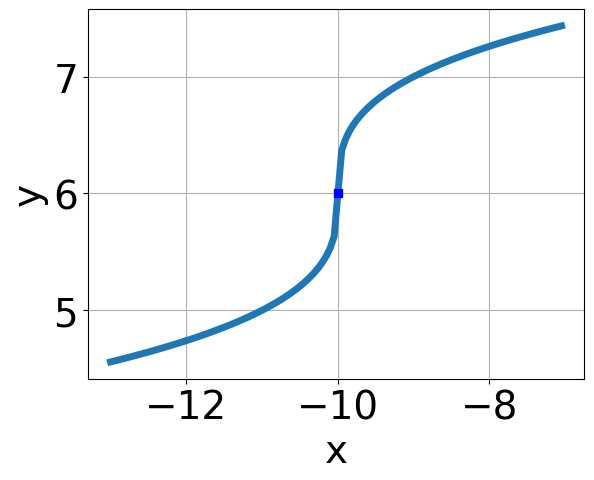
\includegraphics[width = 0.3\textwidth]{../Figures/radicalEquationToGraphCopyBB.png}\item 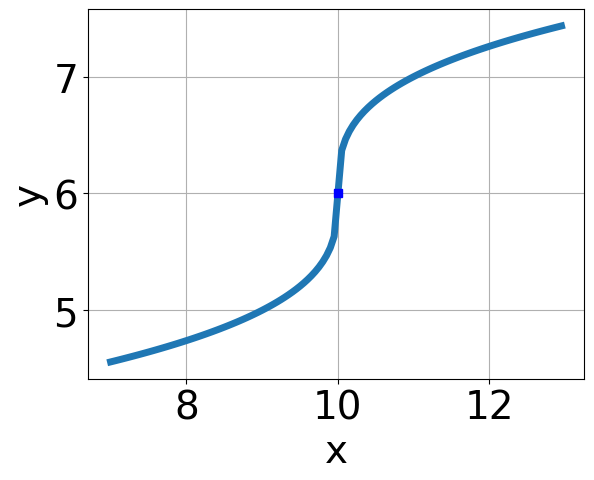
\includegraphics[width = 0.3\textwidth]{../Figures/radicalEquationToGraphCopyCB.png}\item 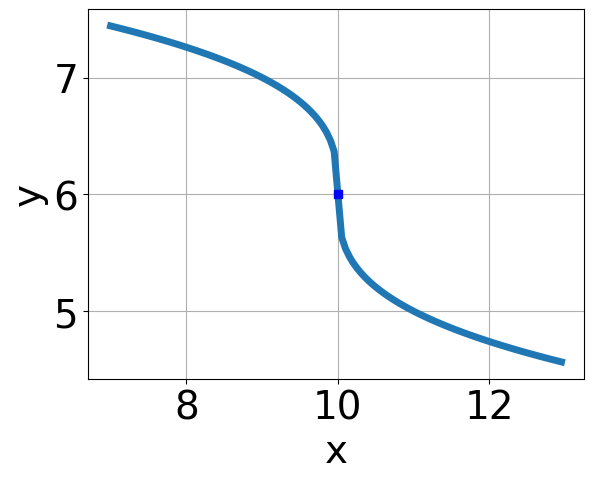
\includegraphics[width = 0.3\textwidth]{../Figures/radicalEquationToGraphCopyDB.png}\end{multicols}\item None of the above.
\end{enumerate} }
\litem{
What is the domain of the function below?\[ f(x) = \sqrt[6]{5 x + 9} \]\begin{enumerate}[label=\Alph*.]
\item \( (-\infty, \infty) \)
\item \( (-\infty, a], \text{where } a \in [-4.5, -0.8] \)
\item \( (-\infty, a], \text{where } a \in [-0.7, 0.6] \)
\item \( [a, \infty), \text{ where } a \in [-3.04, -0.59] \)
\item \( [a, \infty), \text{where } a \in [-1.36, 0.62] \)

\end{enumerate} }
\litem{
Solve the radical equation below. Then, choose the interval(s) that the solution(s) belongs to.\[ \sqrt{32 x^2 + 24} - \sqrt{-76 x} = 0 \]\begin{enumerate}[label=\Alph*.]
\item \( x \in [-1.81,-0.27] \)
\item \( x_1 \in [-0.14, 0.63] \text{ and } x_2 \in [0.4,3.9] \)
\item \( x_1 \in [-2.1, -1.51] \text{ and } x_2 \in [-1.1,0.2] \)
\item \( x \in [-2.1,-1.51] \)
\item \( \text{All solutions lead to invalid or complex values in the equation.} \)

\end{enumerate} }
\litem{
Choose the equation of the function graphed below.
\begin{center}
    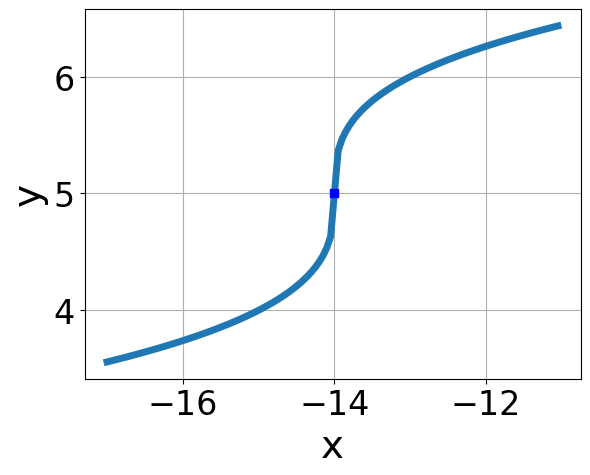
\includegraphics[width=0.5\textwidth]{../Figures/radicalGraphToEquationCopyB.png}
\end{center}
\begin{enumerate}[label=\Alph*.]
\item \( f(x) = \sqrt{x + 14} + 5 \)
\item \( f(x) = - \sqrt{x - 14} + 5 \)
\item \( f(x) = - \sqrt{x + 14} + 5 \)
\item \( f(x) = \sqrt{x - 14} + 5 \)
\item \( \text{None of the above} \)

\end{enumerate} }
\litem{
Solve the radical equation below. Then, choose the interval(s) that the solution(s) belongs to.\[ \sqrt{-6 x - 7} - \sqrt{-3 x + 7} = 0 \]\begin{enumerate}[label=\Alph*.]
\item \( x_1 \in [-4.17, -0.17] \text{ and } x_2 \in [2.33,5.33] \)
\item \( x \in [-0,1] \)
\item \( x \in [-5.67,-1.67] \)
\item \( x_1 \in [-5.67, -1.67] \text{ and } x_2 \in [-1.17,1.83] \)
\item \( \text{All solutions lead to invalid or complex values in the equation.} \)

\end{enumerate} }
\litem{
Solve the radical equation below. Then, choose the interval(s) that the solution(s) belongs to.\[ \sqrt{-48 x^2 - 9} - \sqrt{-42 x} = 0 \]\begin{enumerate}[label=\Alph*.]
\item \( x \in [0.46,0.53] \)
\item \( x_1 \in [0.36, 0.41] \text{ and } x_2 \in [-0.38,1.8] \)
\item \( \text{All solutions lead to invalid or complex values in the equation.} \)
\item \( x \in [0.36,0.41] \)
\item \( x_1 \in [-0.55, -0.35] \text{ and } x_2 \in [-1.34,-0.02] \)

\end{enumerate} }
\litem{
Solve the radical equation below. Then, choose the interval(s) that the solution(s) belongs to.\[ \sqrt{-8 x - 6} - \sqrt{7 x - 7} = 0 \]\begin{enumerate}[label=\Alph*.]
\item \( x_1 \in [-0.78, -0.75] \text{ and } x_2 \in [0.83,1.87] \)
\item \( x \in [-0.93,-0.76] \)
\item \( \text{All solutions lead to invalid or complex values in the equation.} \)
\item \( x \in [0.01,0.41] \)
\item \( x_1 \in [-0.78, -0.75] \text{ and } x_2 \in [-0.84,0.73] \)

\end{enumerate} }
\litem{
Choose the graph of the equation below.\[ f(x) = \sqrt{x + 14} - 6 \]\begin{enumerate}[label=\Alph*.]
\begin{multicols}{2}\item 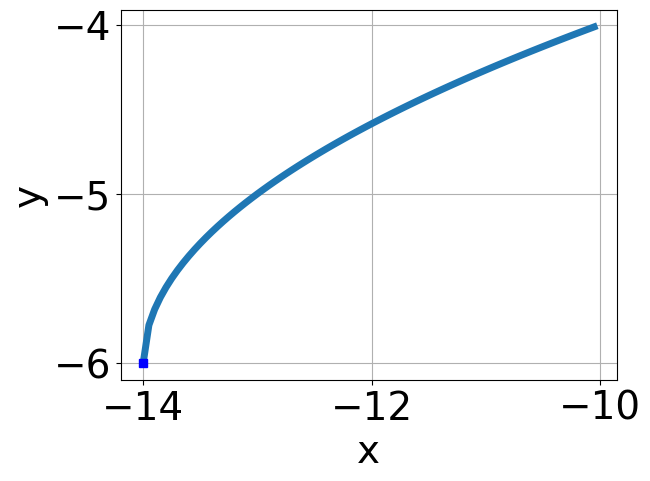
\includegraphics[width = 0.3\textwidth]{../Figures/radicalEquationToGraphAB.png}\item 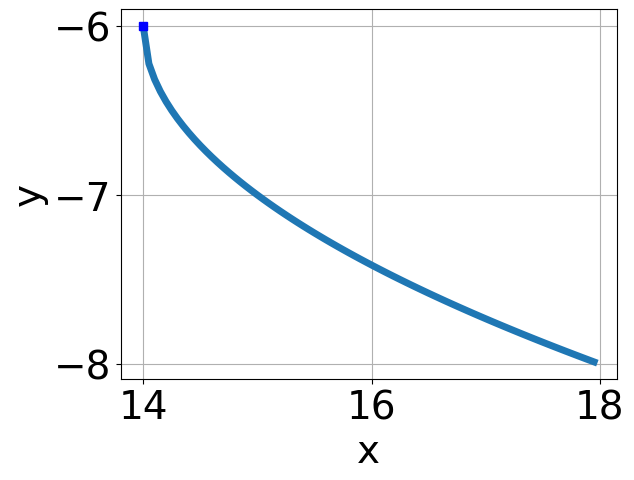
\includegraphics[width = 0.3\textwidth]{../Figures/radicalEquationToGraphBB.png}\item 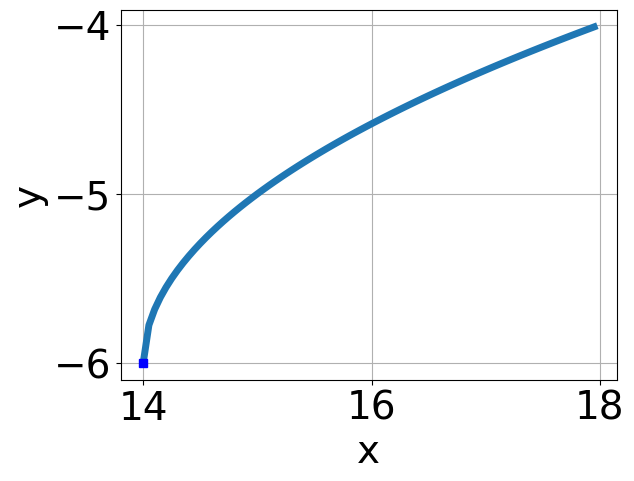
\includegraphics[width = 0.3\textwidth]{../Figures/radicalEquationToGraphCB.png}\item 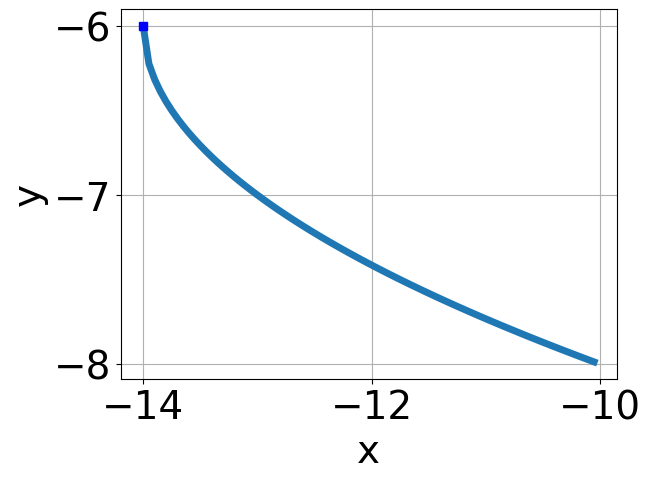
\includegraphics[width = 0.3\textwidth]{../Figures/radicalEquationToGraphDB.png}\end{multicols}\item None of the above.
\end{enumerate} }
\litem{
What is the domain of the function below?\[ f(x) = \sqrt[3]{5 x - 7} \]\begin{enumerate}[label=\Alph*.]
\item \( (-\infty, \infty) \)
\item \( \text{The domain is } (-\infty, a], \text{   where } a \in [0.5, 0.95] \)
\item \( \text{The domain is } (-\infty, a], \text{   where } a \in [1.23, 2.47] \)
\item \( \text{The domain is } [a, \infty), \text{   where } a \in [-0.9, 1.1] \)
\item \( \text{The domain is } [a, \infty), \text{   where } a \in [0.9, 2.8] \)

\end{enumerate} }
\litem{
Choose the equation of the function graphed below.
\begin{center}
    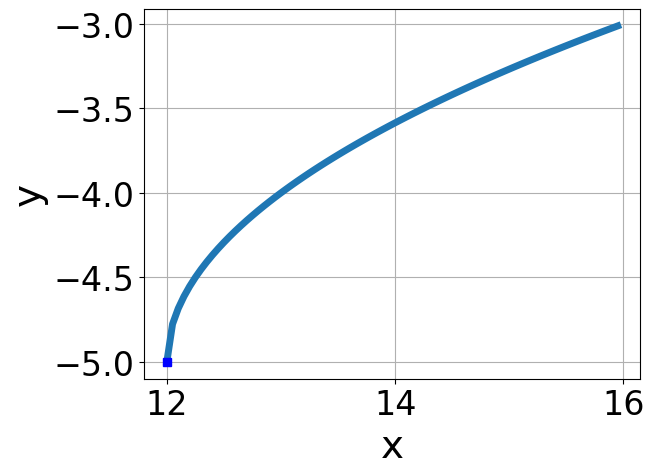
\includegraphics[width=0.5\textwidth]{../Figures/radicalGraphToEquationC.png}
\end{center}
\begin{enumerate}[label=\Alph*.]
\item \( f(x) = - \sqrt[3]{x - 12} - 5 \)
\item \( f(x) = \sqrt[3]{x - 12} - 5 \)
\item \( f(x) = - \sqrt[3]{x + 12} - 5 \)
\item \( f(x) = \sqrt[3]{x + 12} - 5 \)
\item \( \text{None of the above} \)

\end{enumerate} }
\litem{
Choose the graph of the equation below.\[ f(x) = - \sqrt[3]{x + 12} + 3 \]\begin{enumerate}[label=\Alph*.]
\begin{multicols}{2}\item 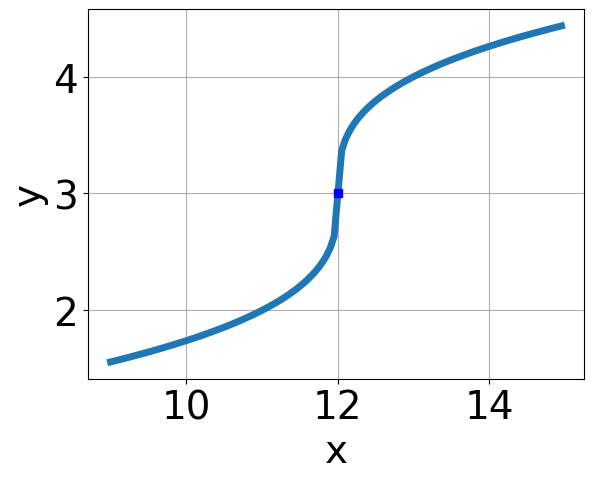
\includegraphics[width = 0.3\textwidth]{../Figures/radicalEquationToGraphCopyAC.png}\item 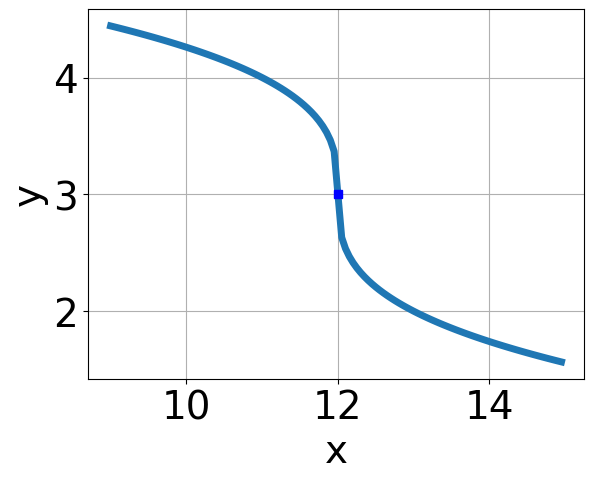
\includegraphics[width = 0.3\textwidth]{../Figures/radicalEquationToGraphCopyBC.png}\item 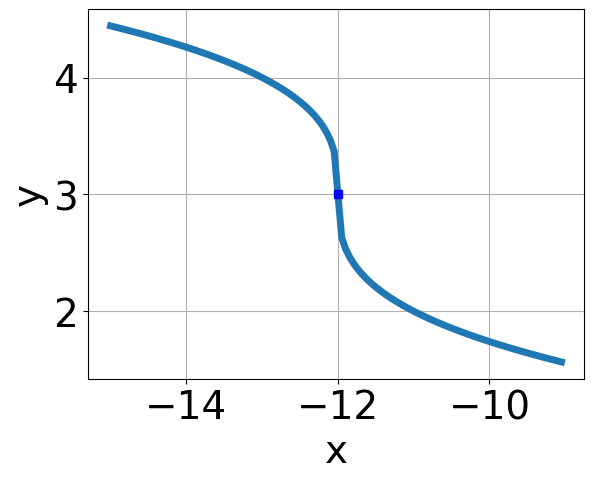
\includegraphics[width = 0.3\textwidth]{../Figures/radicalEquationToGraphCopyCC.png}\item 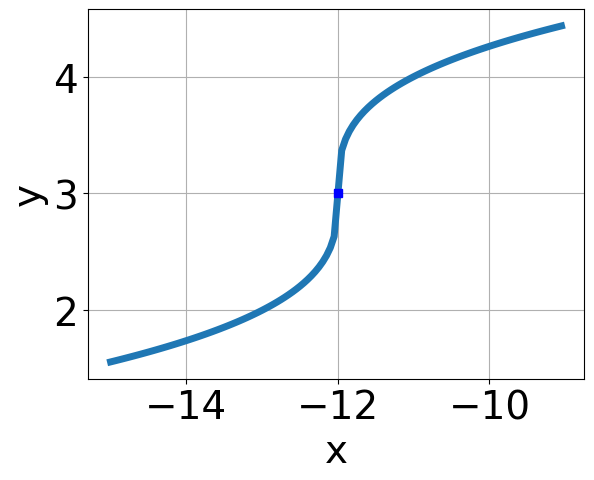
\includegraphics[width = 0.3\textwidth]{../Figures/radicalEquationToGraphCopyDC.png}\end{multicols}\item None of the above.
\end{enumerate} }
\litem{
What is the domain of the function below?\[ f(x) = \sqrt[4]{-4 x - 5} \]\begin{enumerate}[label=\Alph*.]
\item \( [a, \infty), \text{where } a \in [-2.36, -0.83] \)
\item \( (-\infty, \infty) \)
\item \( (-\infty, a], \text{where } a \in [-0.93, -0.64] \)
\item \( (-\infty, a], \text{ where } a \in [-1.43, -0.91] \)
\item \( [a, \infty), \text{where } a \in [-1.11, 1.51] \)

\end{enumerate} }
\litem{
Solve the radical equation below. Then, choose the interval(s) that the solution(s) belongs to.\[ \sqrt{12 x^2 - 14} - \sqrt{38 x} = 0 \]\begin{enumerate}[label=\Alph*.]
\item \( x_1 \in [-0.29, 0.48] \text{ and } x_2 \in [3.5,5.5] \)
\item \( x \in [-0.57,0.19] \)
\item \( x \in [2.68,4.7] \)
\item \( \text{All solutions lead to invalid or complex values in the equation.} \)
\item \( x_1 \in [-0.57, 0.19] \text{ and } x_2 \in [3.5,5.5] \)

\end{enumerate} }
\litem{
Choose the equation of the function graphed below.
\begin{center}
    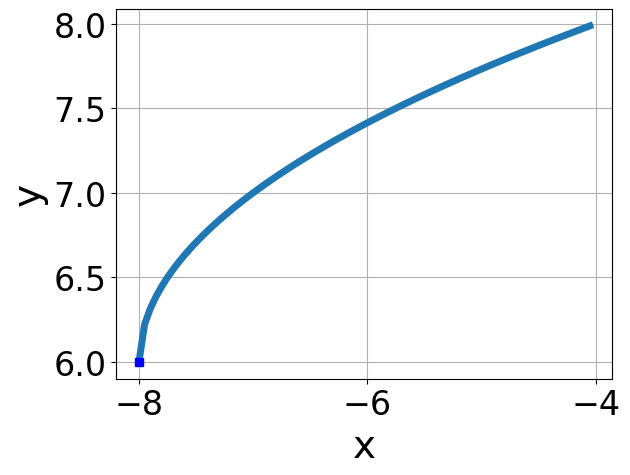
\includegraphics[width=0.5\textwidth]{../Figures/radicalGraphToEquationCopyC.png}
\end{center}
\begin{enumerate}[label=\Alph*.]
\item \( f(x) = - \sqrt{x + 8} + 6 \)
\item \( f(x) = - \sqrt{x - 8} + 6 \)
\item \( f(x) = \sqrt{x - 8} + 6 \)
\item \( f(x) = \sqrt{x + 8} + 6 \)
\item \( \text{None of the above} \)

\end{enumerate} }
\litem{
Solve the radical equation below. Then, choose the interval(s) that the solution(s) belongs to.\[ \sqrt{5 x - 4} - \sqrt{-7 x + 9} = 0 \]\begin{enumerate}[label=\Alph*.]
\item \( x_1 \in [0.78, 0.91] \text{ and } x_2 \in [1.25,1.29] \)
\item \( x_1 \in [0.78, 0.91] \text{ and } x_2 \in [0.84,1.12] \)
\item \( x \in [-0.61,-0.31] \)
\item \( x \in [0.97,1.1] \)
\item \( \text{All solutions lead to invalid or complex values in the equation.} \)

\end{enumerate} }
\litem{
Solve the radical equation below. Then, choose the interval(s) that the solution(s) belongs to.\[ \sqrt{-35 x^2 + 36} - \sqrt{-43 x} = 0 \]\begin{enumerate}[label=\Alph*.]
\item \( \text{All solutions lead to invalid or complex values in the equation.} \)
\item \( x_1 \in [0, 1.05] \text{ and } x_2 \in [-0.2,2.8] \)
\item \( x_1 \in [-1.1, -0.09] \text{ and } x_2 \in [-0.2,2.8] \)
\item \( x \in [-1.1,-0.09] \)
\item \( x \in [1.33,2.34] \)

\end{enumerate} }
\litem{
Solve the radical equation below. Then, choose the interval(s) that the solution(s) belongs to.\[ \sqrt{-4 x - 9} - \sqrt{-5 x + 7} = 0 \]\begin{enumerate}[label=\Alph*.]
\item \( x \in [15,17] \)
\item \( x_1 \in [-7.25, 0.75] \text{ and } x_2 \in [15,17] \)
\item \( \text{All solutions lead to invalid or complex values in the equation.} \)
\item \( x \in [1,4] \)
\item \( x_1 \in [-7.25, 0.75] \text{ and } x_2 \in [0.4,6.4] \)

\end{enumerate} }
\litem{
Choose the graph of the equation below.\[ f(x) = - \sqrt[3]{x + 10} + 7 \]\begin{enumerate}[label=\Alph*.]
\begin{multicols}{2}\item 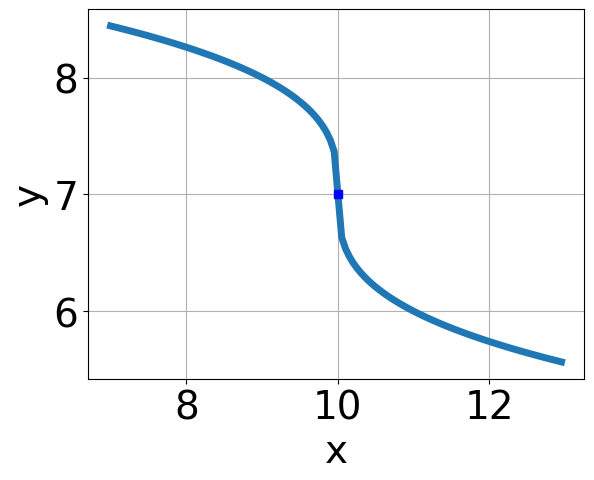
\includegraphics[width = 0.3\textwidth]{../Figures/radicalEquationToGraphAC.png}\item 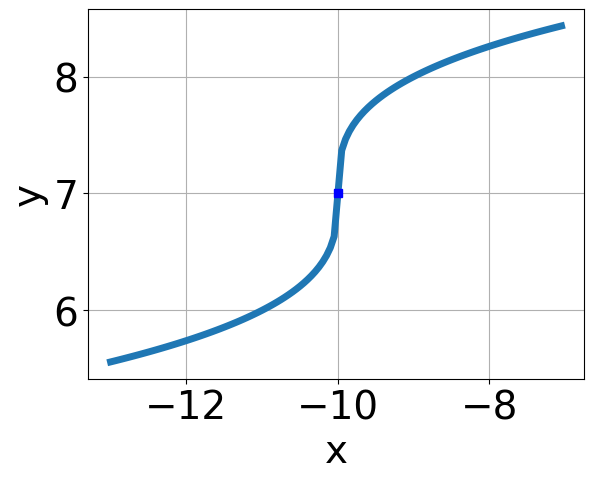
\includegraphics[width = 0.3\textwidth]{../Figures/radicalEquationToGraphBC.png}\item 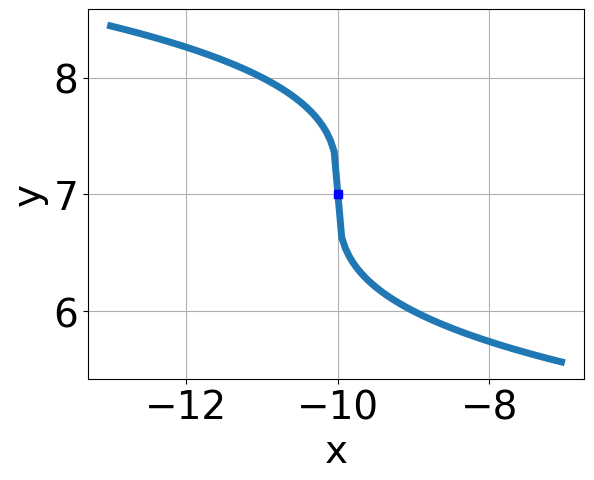
\includegraphics[width = 0.3\textwidth]{../Figures/radicalEquationToGraphCC.png}\item 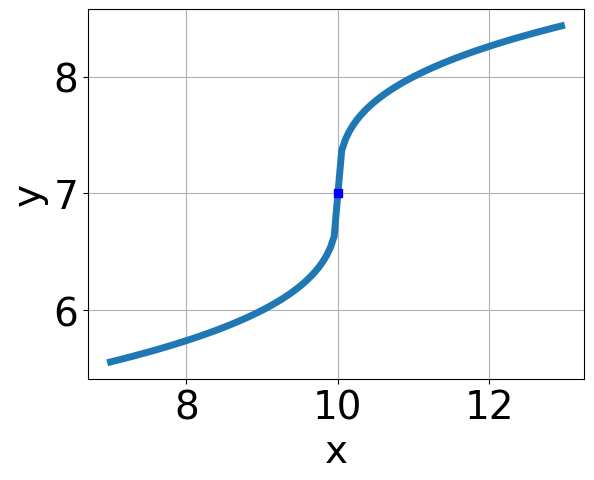
\includegraphics[width = 0.3\textwidth]{../Figures/radicalEquationToGraphDC.png}\end{multicols}\item None of the above.
\end{enumerate} }
\litem{
What is the domain of the function below?\[ f(x) = \sqrt[4]{-6 x - 5} \]\begin{enumerate}[label=\Alph*.]
\item \( [a, \infty), \text{where } a \in [-0.85, -0.18] \)
\item \( (-\infty, \infty) \)
\item \( (-\infty, a], \text{where } a \in [-1.94, -0.87] \)
\item \( [a, \infty), \text{where } a \in [-1.76, -1.11] \)
\item \( (-\infty, a], \text{ where } a \in [-0.98, -0.42] \)

\end{enumerate} }
\end{enumerate}

\end{document}